\documentclass{article}

% Packages
\usepackage[utf8]{inputenc} % For modern characters
\usepackage{microtype} % For sexy kerning
\usepackage{mathtools} % For math stuff
\usepackage{amssymb} % For math symbols
\usepackage{tabularx} % For making tables
\usepackage{fancyhdr} % Use a header
\usepackage{pdfpages} % For including a graphics path

% Set the margins
\usepackage[scale=0.8, top=1in, bottom=1in]{geometry}

% Other front matter
\graphicspath{ {img/} } % Put all graphics in img/
\newcommand{\code}[1]{\texttt{#1}} % More readable for writing inline code.
\newcommand{\p}[1]{\paragraph{#1}} % Easier to type out for paragraph command
\newcommand{\addsection}[1]{\addcontentsline{toc}{section}{#1}} % content lines
\newcommand{\addsubsection}[1]{\addcontentsline{toc}{subsection}{#1}} % content lines
\pagestyle{fancy} % Makes Header Possible
{ %%% Header Set up
	\lhead{} % Set the left header to be blank
	\chead{} % Set the center header to be blank
	% Header for every page except the first two
	\rhead{Ben Foster | Homework 2.4 | May 12, 2015} % Name, assignment, date
}
\setcounter{tocdepth}{2} % Set Table of Contents Depth
\setlength{\parindent}{0pt} % Disable automatic indentation

%%%%%%%%%%%%%%%%%%%%% Begin Document %%%%%%%%%%%%%%%%%%%%%
\begin{document}

{ % Title page, table of contents, and page number setting
	\title{Matrix Algebra Homework 2.4 Applications \\ TMATH 308}
	\author{Ben Foster\thanks{
		Institute of Technology, University of Washington Tacoma} \\
		Instructor: Olga Shatunova}
	\date{May 12, 2015}
	\maketitle
	\thispagestyle{empty} % No page number at bottom
	\clearpage
	
	\pagenumbering{roman}
	\tableofcontents
	\clearpage
	\setcounter{page}{1}
	\pagenumbering{arabic}
}

\section*{Problem 10}
\addsection{First Problem}

The downtown core of Gotham City consists of one-way streets, and the traffic flow has been measured at each intersection. For the city block shown in the figure, the numbers represent the average numbers of vehicles per minute entering and leaving intersections A, B, C, and D during business hours. Let $w = 20$, $x = 20$, $y = 30$, and $z = 25$.

\begin{center}
	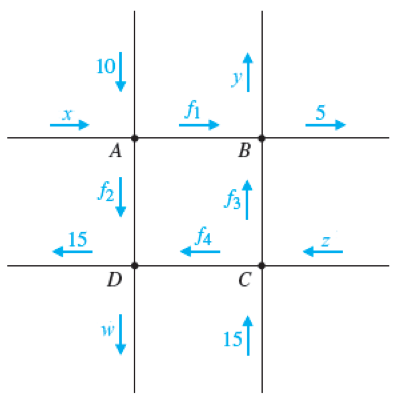
\includegraphics[width=4in]{prob10.jpg}
\end{center}

(a) Set up and solve a system of linear equations to find the possible flows $f_1, ... , f_4$. (Use the parameter $t$ as necessary.) 

\p{Answer} \mbox{} \\
\[ 10 + 20 = f_1 + f_2 \]
\[ 30 + 5 = f_1 + f_3 \]
\[ 15 + 25 = f_3 + f_4 \]
\[ 15 + 20 = f_2 + f_4 \]

\[ f_1 + f_2 = 30 \]
\[ f_1 + f_3 = 35 \]
\[ f_3 + f_4 = 40 \]
\[ f_2 + f_4 = 35 \]

Now we can make a table from the equations:

\begin{center}
\begin{tabular}{ c c c c | c }
	1 & 1 & 0 & 0 & 30 \\
	1 & 0 & 1 & 0 & 35 \\
	0 & 0 & 1 & 1 & 40 \\
	0 & 1 & 0 & 1 & 35 \\
\end{tabular}
\end{center}

In Row Reduced Echelon Form: 

\begin{center}
\begin{tabular}{ c c c c | c }
	1 & 0 & 0 & -1 & -5 \\
	0 & 1 & 0 & 1 & 35 \\
	0 & 0 & 1 & 1 & 40 \\
	0 & 0 & 0 & 0 & 0 \\
\end{tabular}
\end{center}

\[ (f_1,f_2,f_3,f_4) = (t-5,35-t,40-t,t) \]

(b) If traffic is regulated on CD so that $f_4 = 15$ vehicles per minute, what will the average flows on the other streets be? 

\p{Answer} \mbox{} \\
\[ f_4 = t = 15 \]
\[ f_1 = t - 5 = 10 \]
\[ f_2 = 35 - t = 20 \]
\[ f_3 = 40 - t = 25 \]

(c) What are the minimum and maximum possible flows on each street? 

\p{Answer}
Since the streets are one way, then we can't have any negative numbers. After doing a little analysis, the minimum that $f_4$ could be is zero, and we'll have to go to one of the other equations to see what the maximum will be. Looking at the equation for $f_1$, we can see that the minimum for $t$ or $f_4$ can actually be 5 since anything less would cause a negative number. We can't tell the maximum from this equation. Looking at the equation for $f_2$, if $t$ were larger than 35, then we would get a negative number. Looking at the equation for $f_3$, we can see that if $t$ were larger than 40, then we would have a negative number, but we also already know that it can't be larger than 35. Therefore:
\[ 0 \le f_1 \le 30 \]
\[ 0 \le f_2 \le 30 \]
\[ 5 \le f_3 \le 35 \]
\[ 5 \le f_4 \le 35 \]

(d) How would the solution change if all of the directions were reversed?

\p{Answer} \mbox{} \\

If all the directions were reversed, then there would be no effect because they are all one way streets and for each intersection, the two vectors that are going into a specific intersection and the two that are coming out of that same intersection will still either be leaving or going in with the same relation.

\clearpage
\section*{Problem 11}
\addsection{Second Problem}

Consider the following figure.

\begin{center}
	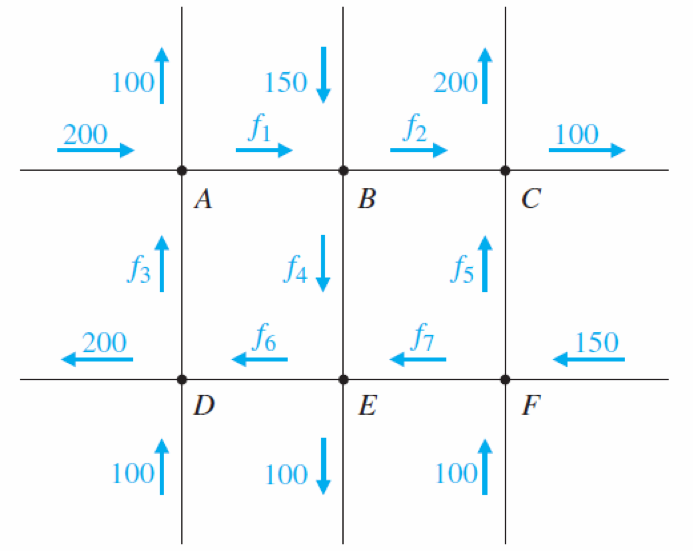
\includegraphics[width=4in]{prob11.jpg}
\end{center}

(a) Set up and solve a system of linear equations to find the possible flows in the network shown in the figure. (Use the parameters s and t as necessary.)

\p{Answer} \mbox{} \\
\[ 200 - 100 = f_1 - f_3 \]
\[ f_1 + 150 = f_2 + f_4 \]
\[ 100 + 200 = f_2 + f_5 \]
\[ 100 - 200 = f_3 - f_6 \]
\[ f_4 + f_7 = f_6 + 100 \]
\[ 100 + 150 = f_5 + f_7 \]

\[ f_1 - f_3 = 100 \]
\[ f_1 - f_2 - f_4 = -150 \]
\[ f_2 + f_5 = 300 \]
\[ f_3 - f_6 = -100 \]
\[ f_4 - f_6 + f_7 = 100 \]
\[ f_5 + f_7 = 250 \]

Now we can make a table from the equations:

\begin{center}
\begin{tabular}{ c c c c c c c | c }
	1 & 0 & -1 & 0 & 0 & 0 & 0 & 100 \\
	1 & -1 & 0 & -1 & 0 & 0 & 0 & -150 \\
	0 & 1 & 0 & 0 & 1 & 0 & 0 & 300 \\
	0 & 0 & 1 & 0 & 0 & -1 & 0 & -100 \\
	0 & 0 & 0 & 1 & 0 & -1 & 1 & 100 \\
	0 & 0 & 0 & 0 & 1 & 0 & 1 & 250 \\
\end{tabular}
\end{center}

In Row Reduced Echelon Form: 

\begin{center}
\begin{tabular}{ c c c c c c c | c }
	1 & 0 & 0 & 0 & 0 & -1 & 0 & 0 \\
	0 & 1 & 0 & 0 & 0 & 0 & -1 & 50 \\
	0 & 0 & 1 & 0 & 0 & -1 & 0 & -100 \\
	0 & 0 & 0 & 1 & 0 & -1 & 1 & 100 \\
	0 & 0 & 0 & 0 & 1 & 0 & 1 & 250 \\
	0 & 0 & 0 & 0 & 0 & 0 & 0 & 0 \\
\end{tabular}
\end{center}

\[ (f_1,f_2,f_3,f_4,f_5,f_6,f_7) = (s, 50 + t, s - 100, 100 - t + s, 250 - t, s, t) \]

(b) Is it possible for $f_1 = 130$ and $f_6 = 140$? [Answer this question first with reference to your solution in part (a) and then directly from the figure.] 

\p{Answer} \mbox{} \\
Looking at the solution from part a, we can see that it is not possible to have $f_1 = 130$ and $f_6 = 140$ because $f_1 = f_6$. If we look at the figure though, we are unable to tell.

\clearpage
\section*{Problem 12}
\addsection{Third Problem}

Determine the current for the given electrical network. (Assume x = 8 and y = 31.)

\begin{center}
	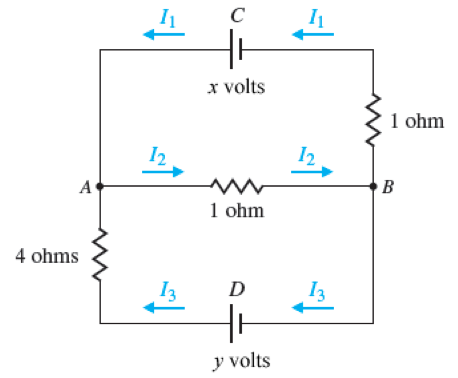
\includegraphics[width=4in]{prob12.jpg}
\end{center}

\p{Answer} \mbox{} \\
From analyzing the picture we get the equations:
\[ I_1 - I_2 + I_3 = 0 \]
\[ I_1 + I_2 = 6 \]
\[ I_2 + 4I_3 = 12 \]
From this we can put these into a matrix:
\begin{center}
\begin{tabular}{ c c c | c }
	1 & -1 & 1 & 0 \\
	1 & 1 & 0 & 6 \\
	0 & 1 & 4 & 12 \\
\end{tabular}
\end{center}
From this, we get the Row Reduced Echelon form:
\begin{center}
\begin{tabular}{ c c c | c }
	1 & 0 & 0 & 2 \\
	0 & 1 & 0 & 4 \\
	0 & 0 & 1 & 2 \\
\end{tabular}
\end{center}
And so: \\
$I_1 = 2$ \\
$I_2 = 4$ \\
$I_3 = 2$

\clearpage
\section*{Problem 5}
\addsection{Fourth Problem}

Balance the chemical equation for the reaction.
\[ FeS_2 +  O_2 \rightarrow Fe_2O_3 + SO_2 \]
First we get our equations: \\
$Fe: 1 + 0 - 2 = 0$ \\
$S: 2 + 0 - 0 = 1$ \\
$ O: 0 + 2 - 3 = 2$ \\
And from this we can get a table:
\begin{center}
\begin{tabular}{ c c c | c }
	1 & 0 & -2 & 0 \\
	2 & 0 & 0 & 1 \\
	0 & 2 & -3 & 2 \\
\end{tabular}
\end{center}
After we get the Row Reduced Echelon Form:
\begin{center}
\begin{tabular}{ c c c | c }
	1 & 0 & 0 & $\frac{1}{2}$ \\
	0 & 1 & 0 & $\frac{11}{8}$ \\
	0 & 0 & 1 & $\frac{1}{4}$ \\
\end{tabular}
\end{center}
Now we just have to multiply each of the answers by 8 so that we don't end up with fractions. \\
first coefficient: 4 \\
second coefficient: 11 \\
third coefficient: 2 \\
fourth coefficient: 8 \\

Therefore:
\[ 4(FeS_2) +  11(O_2) \rightarrow 2(Fe_2O_3) + 8(SO_2) \]

\end{document}
